\documentclass[11pt,a4paper]{article}

\usepackage{mathpazo}
\usepackage{microtype}
\usepackage{url}
\usepackage{verbatim}
\usepackage{graphicx}
\usepackage{titlesec}
\usepackage{float}


\usepackage{tikz}
\usetikzlibrary{external,positioning,through,calc,intersections}
\tikzexternalize[prefix=tikz/]


\textwidth=15cm
\textheight=23cm
\topmargin=18pt
\headheight=0pt
\oddsidemargin=2em
\headsep=0pt
\renewcommand{\baselinestretch}{1.1}
\setlength{\parskip}{0.3\baselineskip plus 1pt minus 1pt}
\parindent=0pt

\begin{document}
\thispagestyle{empty}

\begin{center}

\textbf{\huge Help, My Compass Collapsed!}

\bigskip
\bigskip
\bigskip

\textbf{\LARGE Moti Ben-Ari}

\bigskip

\textbf{\Large Department of Science Teaching}

\bigskip

\textbf{\Large Weizmann Institute of Science}

\bigskip

\url{http://www.weizmann.ac.il/sci-tea/benari/}

\end{center}

\bigskip
\bigskip

\begin{center}
\copyright{}\  2018 by Moti Ben-Ari.
\end{center}

This work is licensed under the Creative Commons Attribution-ShareAlike 3.0 Unported License. To view a copy of this license, visit \url{http://creativecommons.org/licenses/by-sa/3.0/} or send a letter to Creative Commons, 444 Castro Street, Suite 900, Mountain View, California, 94041, USA.

\bigskip

\begin{center}

\includegraphics[width=.2\textwidth]{../by-sa.png}
\end{center}

\newpage

%%%%%%%%%%%%%%%%%%%%%%%%%%%%%%%%%%%%%%%%%%%%%%%%%%%%%%%%%%%%%%%

\section{Fixed compasses and collapsing compasses}

In a modern compass used for geometric constructions the distance between the two legs can be fixed so that it is possible to copy a line segment or a circle from one position to another. I have seen geometry textbooks that present the  construction a perpendicular bisector to a line segment as follows: construct two circles centered at the ends of the line segment such that the radii are \emph{equal} and greater than half the length of the segment (Figure~\ref{fig.bisector} left). We will call such a compass a \emph{fixed compass}.

\begin{figure}[H]
\begin{center}
\begin{tikzpicture}[scale=0.5]
\begin{scope}
\coordinate (A) at (0,0);
\coordinate (B) at (4,0);
\draw (A) node[below left] {$A$} -- (B) node[below right] {$B$};
\fill (A) circle[radius=3pt];
\fill (B) circle[radius=3pt];
\draw[name path=larc] (A) ++(-60:3cm) arc (-60:60:3cm);
\draw[name path=rarc] (B) ++(-120:3cm) arc (-120:-240:3cm);
\path [name intersections={of=larc and rarc,by={b,t}}];
\fill (t) node[above right,xshift=-2pt,yshift=5pt] {$C$} circle[radius=3pt];
\fill (b) node[below left,xshift=2pt,yshift=-5pt] {$D$} circle[radius=3pt];
\draw ($ (b) ! 1.2 ! (t)$) -- ($ (t) ! 1.2 ! (b)$);
\end{scope}
\begin{scope}[xshift=12cm]
\coordinate (A) at (0,0);
\coordinate (B) at (4,0);
\draw (A) node[below left] {$A$} -- (B) node[below right] {$B$};
\fill (A) circle[radius=3pt];
\fill (B) circle[radius=3pt];
\draw[name path=larc] (A) ++(-80:4cm) arc (-80:80:4cm);
\draw[name path=rarc] (B) ++(-100:4cm) arc (-100:-260:4cm);
\path [name intersections={of=larc and rarc,by={b,t}}];
\fill (t) node[above right,xshift=-2pt,yshift=3pt] {$C$} circle[radius=3pt];
\fill (b) node[below left,xshift=2pt,yshift=-3pt] {$D$}circle[radius=3pt];
\draw ($ (b) ! 1.2 ! (t)$) -- ($ (t) ! 1.2 ! (b)$);
\end{scope}
\end{tikzpicture}
\caption{Perpendicular bisector.}\label{fig.bisector}
\end{center}
\end{figure}
\vspace*{-3ex}
Euclid used a \emph{collapsing compass} whose legs fold up when the compass is lifted off the paper. Teachers often use a collapsing compass consisting of a piece of chalk tied to a string. It is impossible to maintain a fixed radius when the chalk is removed from the blackboard. Figure~\ref{fig.bisector} (right) shows how to construct a perpendicular bisector with a collapsing compass: the length of the segment $AB$ is, of course, equal to the length of the segment $BA$, so the radii of the two circles are equal and there is no need to copy a line segment from one position to another.

The proof that the line constructed is, in fact, the perpendicular bisector is not at all elementary because relatively advanced concepts like congruent triangles have to be used. However, the proof that the same construction results in an equilateral triangle is very simple (Figure~\ref{fig.equilateral} right).

The length of $AC$ equals the length of $AB$ since they are radii of the same circle, and for the same reason the length of $BC$ is equal to the length of $BA$. We have:
\[
AC=AB=BA=BC\,.
\]
Figure~\ref{fig.equilateral} (left) shows that for the construction with the fixed compass the triangle will be isosceles, but not necessarily equilateral.
\begin{figure}[H]
\begin{center}
\begin{tikzpicture}[scale=0.5]
\begin{scope}
\coordinate (A) at (0,0);
\coordinate (B) at (4,0);
\draw (A) node[below left] {$A$} -- (B) node[below right] {$B$};
\fill (A) circle[radius=3pt];
\fill (B) circle[radius=3pt];
\draw[name path=larc] (A) ++(-60:3cm) arc (-60:60:3cm);
\draw[name path=rarc] (B) ++(-120:3cm) arc (-120:-240:3cm);
\path [name intersections={of=larc and rarc,by={b,t}}];
\fill (t) node[above right,xshift=-2pt,yshift=5pt] {$C$} circle[radius=3pt];
\fill (b) node[below left,xshift=2pt,yshift=-5pt] {$D$} circle[radius=3pt];
\draw (A) -- (t);
\draw (B) -- (t);
\end{scope}
\begin{scope}[xshift=12cm]
\coordinate (A) at (0,0);
\coordinate (B) at (4,0);
\draw (A) node[below left] {$A$} -- (B) node[below right] {$B$};
\fill (A) circle[radius=3pt];
\fill (B) circle[radius=3pt];
\draw[name path=larc] (A) ++(-80:4cm) arc (-80:80:4cm);
\draw[name path=rarc] (B) ++(-100:4cm) arc (-100:-260:4cm);
\path [name intersections={of=larc and rarc,by={b,t}}];
\fill (t) node[above right,xshift=-2pt,yshift=3pt] {$C$} circle[radius=3pt];
\fill (b) node[below left,xshift=2pt,yshift=-3pt] {$D$}circle[radius=3pt];
\draw (A) -- (t);
\draw (B) -- (t);
\end{scope}
\end{tikzpicture}
\caption{Equilateral triangle.}\label{fig.equilateral}
\end{center}
\end{figure}
\vspace*{-4ex}
This construction of an equilateral triangle is the first proposition in Euclid's \emph{Elements}. The second proposition shows how to copy a given line segment $AB$ to a segment of the same length, one of whose end points is a given point $C$. Using this construction, we can also construct a circle centered at $C$ with radius $AB$. As we shall see, the construction in the second proposition can be done with a collapsing compass; therefore, any construction that uses a fixed compass can also be done using a collapsing compass.

In a fascinating article, Godfried Toussaint \cite{toussaint} showed that many \emph{incorrect} constructions for this proposition have been given. In fact, it was Euclid who gave a correct construction! In this document, I give a step-by-step presentation of Euclid's construction and the proof of its correctness. Then I show an incorrect construction that can be found even in modern textbooks. Next I survey constructions using tools that are more restricted or more complex than a straightedge and compass. Finally, to show that diagrams cannot be trusted, I present a proof that \emph{all} triangles are isosceles.

%%%%%%%%%%%%%%%%%%%%%%%%%%%%%%%%%%%%%%%%%%%%%%%%%%%%%%%%%%%%%%%

\section{Euclid's construction for copying a line segment}

\textbf{Theorem (Compass Equivalency Theorem):} Given a line segment $AB$ and a point $C$ (Figure~\ref{fig.ce-1} left), a line segment whose length is equal to the length of $AB$ can be constructed (using a collapsing compass) at $C$.
\begin{figure}[H]
\begin{center}
\begin{tikzpicture}[scale=0.5]
\begin{scope}
\coordinate (C) at (0,0);
\coordinate (A) at (2.5,0);
\coordinate (B) at (5.5,2);
\draw (A) node[below,xshift=-2pt,yshift=-2pt] {$A$} -- (B) node[right] {$B$};
\fill (A) circle[radius=3pt];
\fill (B) circle[radius=3pt];
\fill (C) node[below,xshift=2pt,yshift=-2pt] {$C$} circle[radius=3pt];
\end{scope}
\begin{scope}[xshift=12cm]
\coordinate (C) at (0,0);
\coordinate (A) at (2.5,0);
\coordinate (B) at (5.5,2);
\draw (A) node[below,xshift=-2pt,yshift=-2pt] {$A$} -- (B) node[right] {$B$};
\fill (A) circle[radius=3pt];
\fill (B) circle[radius=3pt];
\fill (C) node[below,xshift=2pt,yshift=-2pt] {$C$} circle[radius=3pt];
\draw (A) -- (C);
\path[name path=larc] (C) ++(-70:2.5cm) arc (-70:70:2.5cm);
\path[name path=rarc] (A) ++(-110:2.5cm) arc (-110:-250:2.5cm);
\path [name intersections={of=larc and rarc,by={d,D}}];
\fill (D) node[above] {$D$} circle[radius=3pt];
\draw (A) -- (D);
\draw (C) -- (D);
\end{scope}
\end{tikzpicture}
\caption{Copy line $AB$ to the point $C$. Construct an equilateral triangle on $AC$.}\label{fig.ce-1}
\end{center}
\end{figure}

\newpage

\textbf{Construction:}
\begin{itemize}
\item Construct the line segment from $A$ to $C$.
\item Construct an equilateral triangle whose base is $AC$. Label the third vertex $D$ (Figure~\ref{fig.ce-1} right). By Euclid's first proposition, the triangle can be constructed using a collapsing compass.
\item Construct a ray from $D$ through $A$ and a ray from $D$ through $C$ (Figure~\ref{fig.ce-2} left).
\item Construct a circle centered at $A$ with radius $AB$. Label the intersection of the circle and the ray $DA$ by $E$ (Figure~\ref{fig.ce-2} right).
\item Construct a circle centered at $D$ with radius $DE$. Label the intersection of the circle and the ray $DC$ by $F$ (Figure~\ref{fig.ce-3}).
\item The length of the line segment $CF$ is equal to the length of $AB$.
\end{itemize}
\begin{figure}[H]
\begin{center}
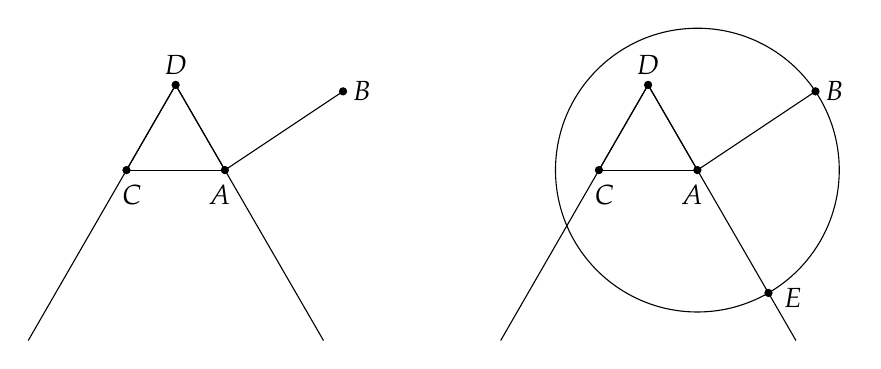
\begin{tikzpicture}[scale=0.5]
\begin{scope}
\coordinate (C) at (0,0);
\coordinate (A) at (2.5,0);
\coordinate (B) at (5.5,2);
\draw (A) node[below,xshift=-2pt,yshift=-2pt] {$A$} -- (B) node[right] {$B$};
\fill (A) circle[radius=3pt];
\fill (B) circle[radius=3pt];
\fill (C) node[below,xshift=2pt,yshift=-2pt] {$C$} circle[radius=3pt];
\draw (A) -- (C);
\path[name path=larc] (C) ++(-70:2.5cm) arc (-70:70:2.5cm);
\path[name path=rarc] (A) ++(-110:2.5cm) arc (-110:-250:2.5cm);
\path [name intersections={of=larc and rarc,by={d,D}}];
\fill (D) node[above] {$D$} circle[radius=3pt];
\draw (A) -- (D);
\draw (C) -- (D);
\draw[name path=ray2] (D) -- ($ (D) ! 3 ! (C) $);
\draw[name path=ray1] (D) -- ($ (D) ! 3 ! (A) $);
\end{scope}
\begin{scope}[xshift=12cm]
\coordinate (C) at (0,0);
\coordinate (A) at (2.5,0);
\coordinate (B) at (5.5,2);
\draw (A) node[below,xshift=-2pt,yshift=-2pt] {$A$} -- (B) node[right] {$B$};
\fill (A) circle[radius=3pt];
\fill (B) circle[radius=3pt];
\fill (C) node[below,xshift=2pt,yshift=-2pt] {$C$} circle[radius=3pt];
\draw (A) -- (C);
\path[name path=larc] (C) ++(-70:2.5cm) arc (-70:70:2.5cm);
\path[name path=rarc] (A) ++(-110:2.5cm) arc (-110:-250:2.5cm);
\path [name intersections={of=larc and rarc,by={d,D}}];
\fill (D) node[above] {$D$} circle[radius=3pt];
\draw (A) -- (D);
\draw (C) -- (D);
\draw[name path=ray2] (D) -- ($ (D) ! 3 ! (C) $);
\draw[name path=ray1] (D) -- ($ (D) ! 3 ! (A) $);
\node[draw,circle through=(B),name path=c1] at (A) {};
\path [name intersections={of=c1 and ray1,by={E,e}}];
\fill (E) node[right,xshift=2pt,yshift=-2pt] {$E$} circle[radius=3pt];
\end{scope}
\end{tikzpicture}
\caption{Rays from $D$ through $A,C$. A circle centered at $A$} \label{fig.ce-2}
\end{center}
\end{figure}
\vspace*{-2ex}
\textbf{Proof:} $DC=DA$ because they are edges of an equilateral triangle. $AE=AB$ because they are radii of the same circle centered at $A$. $DF=DE$ because they are radii of the same circle centered at $D$. Therefore, the length of the line segment $CF$ is:
\[
CF=DF-DC=DE-DC=DE-DA=AE=AB\,.
\]
\begin{figure}[H]
\begin{center}
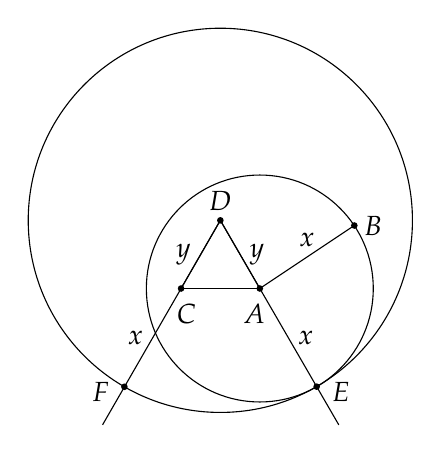
\begin{tikzpicture}[scale=0.4]
\coordinate (C) at (0,0);
\coordinate (A) at (2.5,0);
\coordinate (B) at (5.5,2);
\draw (A) node[below,xshift=-2pt,yshift=-2pt] {$A$} -- node[above] {$x$} (B) node[right] {$B$};
\fill (A) circle[radius=3pt];
\fill (B) circle[radius=3pt];
\fill (C) node[below,xshift=2pt,yshift=-2pt] {$C$} circle[radius=3pt];
\draw (A) -- (C);
\path[name path=larc] (C) ++(-70:2.5cm) arc (-70:70:2.5cm);
\path[name path=rarc] (A) ++(-110:2.5cm) arc (-110:-250:2.5cm);
\path [name intersections={of=larc and rarc,by={d,D}}];
\fill (D) node[above] {$D$} circle[radius=3pt];
\draw (A) -- node[right] {$y$} (D);
\draw (C) -- node[left] {$y$} (D);
\draw[name path=ray2] (D) -- ($ (D) ! 3 ! (C) $);
\draw[name path=ray1] (D) -- ($ (D) ! 3 ! (A) $);
\node[draw,circle through=(B),name path=c1] at (A) {};
\path [name intersections={of=c1 and ray1,by={E,e}}];
\fill (E) node[right,xshift=2pt,yshift=-2pt] {$E$} circle[radius=3pt];
\node[draw,circle through=(E),name path=c2] at (D) {};
\path [name intersections={of=c2 and ray2,by={F,f}}];
\fill (F) node[left,xshift=-2pt,yshift=-2pt] {$F$} circle[radius=3pt];
\path (A) -- node[right] {$x$} (E);
\path (C) -- node[left] {$x$} (F);
\end{tikzpicture}
\caption{A circle centered at $D$ with radius $DE$. $CF=AE=AB$.}\label{fig.ce-3}
\end{center}
\end{figure}

%%%%%%%%%%%%%%%%%%%%%%%%%%%%%%%%%%%%%%%%%%%%%%%%%%%%%%%%%%%%%%%
\newpage

\section{An erroneous construction for copying a line segment}\label{s.erroneous}

The following presentation is based on \cite{rusty}.

\textbf{Theorem (Compass Equivalency Theorem):} Given a line segment $AB$ and a point $C$ (Figure~\ref{fig.rusty-1} left), a line segment whose length is equal to the length of $AB$ can be constructed (using a collapsing compass) at $C$.

\begin{figure}[H]
\begin{center}
\begin{tikzpicture}[scale=0.5]
\begin{scope}
\coordinate (C) at (-2,0);
\coordinate (A) at (2.5,0);
\coordinate (B) at (4.5,1.5);
\draw (A) node[below,xshift=-2pt,yshift=-2pt] {$A$} -- (B) node[right] {$B$};
\fill (A) circle[radius=3pt];
\fill (B) circle[radius=3pt];
\fill (C) node[below,xshift=2pt,yshift=-2pt] {$C$} circle[radius=3pt];
\end{scope}
\begin{scope}[xshift=12cm]
\coordinate (C) at (-2,0);
\coordinate (A) at (2.5,0);
\coordinate (B) at (4.5,1.5);
\draw (A) node[below,xshift=-2pt,yshift=-2pt] {$A$} -- (B) node[right] {$B$};
\fill (A) circle[radius=3pt];
\fill (B) circle[radius=3pt];
\fill (C) node[below,xshift=2pt,yshift=-2pt] {$C$} circle[radius=3pt];
\node[draw,circle through=(B),name path=c1] at (A) {};
\end{scope}
\end{tikzpicture}
\caption{Copy $AB$ to point $C$. A circle centered at $A$ with radius $AB$.}\label{fig.rusty-1}
\end{center}
\end{figure}

\vspace*{-4ex}

\textbf{Construction:}
\begin{itemize}
\item Construct a circle centered at $A$ with radius $AB$ (Figure~\ref{fig.rusty-1} right).
\item Construct a circle centered at $A$ with radius $AC$ and a circle centered at $C$ with radius $AC=CA$. Label the intersections of the two circles $E,F$. Label the intersection of the circle centered at $C$ and the circle centered at $A$ by $D$ (Figure~\ref{fig.rusty-2}).
\begin{figure}[H]	
\begin{center}
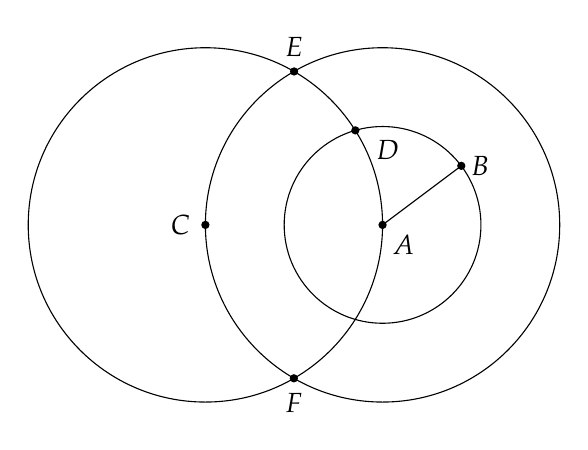
\begin{tikzpicture}[scale=0.5]
\coordinate (C) at (-2,0);
\coordinate (A) at (2.5,0);
\coordinate (B) at (4.5,1.5);
\draw (A) node[below right] {$A$} -- (B) node[right] {$B$};
\fill (A) circle[radius=3pt];
\fill (B) circle[radius=3pt];
\fill (C) node[left,xshift=-2pt] {$C$} circle[radius=3pt];
\node[draw,circle through=(B),name path=c1] at (A) {};
\node[draw,circle through=(C),name path=c2] at (A) {};
\node[draw,circle through=(A),name path=c3] at (C) {};
\path [name intersections={of=c1 and c3,by={D,f}}];
\path [name intersections={of=c2 and c3,by={E,F}}];
\fill (D) node[below right,xshift=4pt] {$D$} circle[radius=3pt];
\fill (E) node[above,yshift=2pt] {$E$} circle[radius=3pt];
\fill (F) node[below,yshift=-2pt] {$F$} circle[radius=3pt];
\end{tikzpicture}
\caption{Circles centered at $A,C$ with radii $AC=CA$.}\label{fig.rusty-2}
\end{center}
\end{figure}
\vspace*{-5ex}
\item Construct a circle centered at $E$ with radius $ED$. Label the intersection of this circle with the circle centered at $C$ by $G$ (Figure~\ref{fig.rusty-3}).
\item The length of the line segment $GC$ is equal to the length of $AB$.
\end{itemize}
Convince yourself that the construction can be carried by using a collapsing compass.

The proof that $AB=GC$ can be found in \cite{rusty}. This is done by showing that the two triangles denoted by dashed lines are congruent so $GC=DA=AB$. The proof is much longer than Euclid's and uses advanced concepts unlike Euclid's proof that depends only on: all radii of a circle are equal as are all sides of an equilateral triangle.
\begin{figure}[H]
\begin{center}
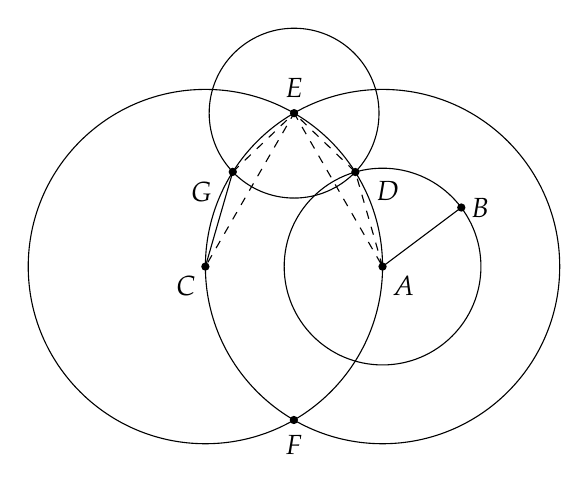
\begin{tikzpicture}[scale=0.5]
\coordinate (C) at (-2,0);
\coordinate (A) at (2.5,0);
\coordinate (B) at (4.5,1.5);
\draw (A) node[below right] {$A$} -- (B) node[right] {$B$};
\fill (A) circle[radius=3pt];
\fill (B) circle[radius=3pt];
\fill (C) node[below left] {$C$} circle[radius=3pt];
\node[draw,circle through=(B),name path=c1] at (A) {};
\node[draw,circle through=(C),name path=c2] at (A) {};
\node[draw,circle through=(A),name path=c3] at (C) {};
\path [name intersections={of=c1 and c3,by={D,f}}];
\path [name intersections={of=c2 and c3,by={E,F}}];
\fill (D) node[below right,xshift=4pt] {$D$} circle[radius=3pt];
\fill (E) node[above,yshift=2pt] {$E$} circle[radius=3pt];
\fill (F) node[below,yshift=-2pt] {$F$} circle[radius=3pt];
\node[draw,circle through=(D),name path=c4] at (E) {};
\path [name intersections={of=c2 and c4,by={g,G}}];
\fill (G) node[below left,xshift=-4pt] {$G$} circle[radius=3pt];
\draw (C) -- (G);
\draw[dashed] (G) -- (E) -- (C);
\draw[dashed] (A) -- (D) -- (E) -- cycle;
\end{tikzpicture}
\caption{A circle centered at $E$ with radius $ED$. Equal line segments $GC=DA=AB$.}\label{fig.rusty-3}
\end{center}
\end{figure}
\vspace*{-3ex}
Look closely at the proof in \cite{rusty} that $AB=GC$ and find the error. The answer: there isn't any error in the proof! The problem arises from a different source: the equality $AB=GC$ holds only when the length of $AB$ is less that the length of $AC$. In contrast, Euclid's construction and proof are true independent of the relative lengths of  $AB$ and $AC$, and of the position of the point $C$ relative to the line segment $AB$ (\cite{toussaint}).


%%%%%%%%%%%%%%%%%%%%%%%%%%%%%%%%%%%%%%%%%%%%%%%%%%%%%%%%%%%%%%%

\section{Exploring the constructions with GeoGebra}

GeoGebra (\url{https://www.geogebra.org/}) is an interactive environment for studying mathematics. I have prepared GeoGebra files for the two constructions: 
\begin{center}
\texttt{compass-equivalency.ggb, rusty-compass.ggb}.
\end{center}
The points $A,B,C$ can be moved around on the screen to see how the diagram changes. You can use the measurement tool to check if the lengths of the line segments are equal.

\textbf{Note:} For Euclid's construction, if you start with $AB<AC$, move $C$ so that $AB>AC$ and then back, the display becomes corrupted. The reason is that whenever $AB<AC$, the ray $DA$ intersects the circle centered at $A$ in two points, but when returning back to $AB<AC$, one intersection point is lost. To work around this problem, I have prepared two version of the files for Euclid's construction.

%%%%%%%%%%%%%%%%%%%%%%%%%%%%%%%%%%%%%%%%%%%%%%%%%%%%%%%%%%%%%%%

\section{A ``simpler'' construction for copying a line segment}

Given a line segment $AB$ and a point $C$, if we can build a parallelogram with these three points as its vertices, we obtain a line segment with $C$ at one end whose length is equal to the length of $AB$ (Figure~\ref{fig.parallel-1} left). This construction can be found in \cite[pp. 207--208]{roads}.
\begin{figure}[H]
\begin{center}
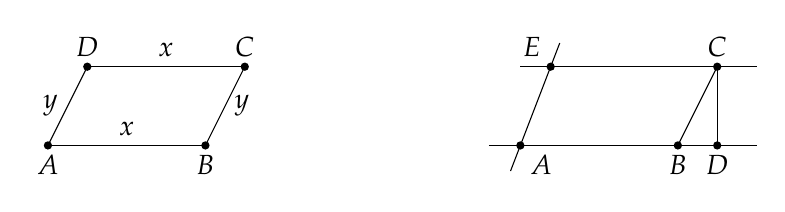
\begin{tikzpicture}[scale=0.5]
\begin{scope}
\coordinate (A) at (0,0);
\coordinate (B) at (4,0);
\coordinate (C) at (5,2);
\draw (A) -- (B);
\path (A) -- node[above] {$x$} (B);
\fill (A) node[below] {$A$} circle[radius=3pt];
\fill (B) node[below] {$B$} circle[radius=3pt];
\fill (C) node[above] {$C$} circle[radius=3pt];
\draw (B) -- node[right] {$y$} (C);
\coordinate (D) at ($(C)+(-40mm,0cm)$);
\draw (D) -- node[above] {$x$} (C);
\draw (A) -- node[left] {$y$} (D);
\fill (D) node[above] {$D$} circle[radius=3pt];
\end{scope}
\begin{scope}[xshift=12cm]
\coordinate (A) at (0,0);
\coordinate (B) at (4,0);
\coordinate (C) at (5,2);
\draw ($ (B) ! 1.2 ! (A) $) -- ($ (A) ! 1.5 ! (B) $);
\path (A) -- (B);
\fill (A) node[below right] {$A$} circle[radius=3pt];
\fill (B) node[below] {$B$} circle[radius=3pt];
\fill (C) node[above] {$C$} circle[radius=3pt];
\draw (B) -- (C);
\draw[name path=ray1] ($(C)+(-5cm,0cm)$) -- ($(C)+(1cm,0cm)$);
\draw[name path=ray2] ($(A)+(-.25,-.65)$) -- ($(A)+(1,2.6)$);
\path [name intersections={of=ray1 and ray2,by={E}}];
\fill (E) node[above left] {$E$} circle[radius=3pt];
\coordinate (D) at (C |- B);
\draw (C) -- (D);
\fill (D) node[below] {$D$} circle[radius=3pt];
\end{scope}
\end{tikzpicture}
\caption{A parallelogram $DC=AB$. Constructing the parallelogram.}\label{fig.parallel-1}
\end{center}
\end{figure}
\vspace*{-4ex}
\textbf{Construction:} (Figure~\ref{fig.parallel-1}, right)
\begin{itemize}
\item Construct the line segment from $B$ to $C$.
\item Construct a perpendicular from $C$ to the line containing the line segment $AB$. Label their intersection by $D$.
\item Construct a perpendicular to the line segment $CD$ at $C$. This line is parallel to $AB$.
\item Use a similar method to construct a line parallel to $BC$ through $A$. Label the intersection of the two lines that we constructed by $E$.
\item The length of the line segment $EC$ is equal to the length of $AB$.
\end{itemize}
We have to check that it is possible to construct the parallelogram with a collapsing compass. The only construction needed is that of a perpendicular from an given point to a line that contains a given line segment (Figure~\ref{fig.perp-1}).
\begin{figure}[H]
\begin{center}
\begin{tikzpicture}[scale=0.5]
\coordinate (A) at (0,0);
\coordinate (B) at (4,0);
\coordinate (C) at (5,2);
\draw ($ (B) ! 1.5 ! (A) $) -- ($ (A) ! 1.5 ! (B) $);
\fill (A) node[below] {$A$} circle[radius=3pt];
\fill (B) node[below] {$B$} circle[radius=3pt];
\fill (C) node[right] {$C$} circle[radius=3pt];
\end{tikzpicture}
\caption{A perpendicular from $C$ to the line containing the segment $AB$.}\label{fig.perp-1}
\end{center}
\end{figure}
\vspace*{-4ex}
Construct a circle centered at $C$ with a radius that is greater than the distance of $C$ from the line (Figure~\ref{fig.perp-2}).
\begin{figure}[H]
\begin{center}
\begin{tikzpicture}[scale=0.5]
\coordinate (A) at (0,0);
\coordinate (B) at (4,0);
\coordinate (C) at (5,2);
\draw[name path=ray] ($ (B) ! 1.5 ! (A) $) -- ($ (A) ! 2.5 ! (B) $);
\fill (A) node[below] {$A$} circle[radius=3pt];
\fill (B) node[below] {$B$} circle[radius=3pt];
\fill (C) node[right] {$C$} circle[radius=3pt];
\draw[name path=arc] (C) ++(-160:3.5cm) arc (-160:-20:3.5cm);
\path [name intersections={of=arc and ray,by={D,E}}];
\fill (D) node[below left] {$D$} circle[radius=3pt];
\fill (E) node[below right] {$E$} circle[radius=3pt];
\end{tikzpicture}
\caption{$D$ and $E$ are at equal distances from $C$.}\label{fig.perp-2}
\end{center}
\end{figure}
\vspace*{-4ex}
Construct the perpendicular bisector of $DE$ through $C$ (Figure~\ref{fig.perp-3}). $CD = CE$ because they are radii of the same circle and the construction can be done with a collapsing compass.

Why didn't Euclid use this construction? As we mentioned earlier, the proof that the line constructed is a perpendicular bisector is not at all easy, while the proof of Euclid's proof is very easy and depends only on a one simple proposition.
\begin{figure}[H]
\begin{center}
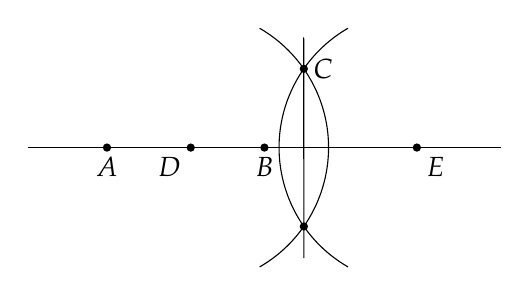
\begin{tikzpicture}[scale=0.5]
\coordinate (A) at (0,0);
\coordinate (B) at (4,0);
\coordinate (C) at (5,2);
\draw[name path=ray] ($ (B) ! 1.5 ! (A) $) -- ($ (A) ! 2.5 ! (B) $);
\fill (A) node[below] {$A$} circle[radius=3pt];
\fill (B) node[below] {$B$} circle[radius=3pt];
\fill (C) node[right] {$C$} circle[radius=3pt];
\path[name path=arc] (C) ++(-160:3.5cm) arc (-160:-20:3.5cm);
\path [name intersections={of=arc and ray,by={D,E}}];
\fill (D) node[below left] {$D$} circle[radius=3pt];
\fill (E) node[below right] {$E$} circle[radius=3pt];
\draw[name path=larc] (D) ++(-60:3.5cm) arc (-60:60:3.5cm);
\draw[name path=rarc] (E) ++(-120:3.5cm) arc (-120:-240:3.5cm);
\path [name intersections={of=larc and rarc,by={b,t}}];
\fill (b) circle[radius=3pt];
\draw ($ (b) ! 1.2 ! (t)$) -- ($ (t) ! 1.2 ! (b)$);
\end{tikzpicture}
\caption{A perpendicular to the line containing $AB$ through $C$.}\label{fig.perp-3}
\end{center}
\end{figure}


%%%%%%%%%%%%%%%%%%%%%%%%%%%%%%%%%%%%%%%%%%%%%%%%%%%%%%%%%%%%%%%

\section{Restrictions and extensions of the straightedge and compass}

We have seen that whatever can be constructed with a straightedge and a fixed compass can be constructed with a straightedge and a collapsing compass. Mathematicians have studied additional restrictions on constructions:

\begin{itemize}
\item Any construction that can be done using a straightedge and compass can be carried out using only a compass! If a straightedge is not used, we won't see any lines, but two points define a line, so it is not really necessary to actually see it. For example, given two points $A,B$, a point $C$ can be constructed so that its distance from $A$ is the same as its distance from $B$ (Figure~\ref{fig.mm}). We have constructed an equilateral triangle with three sides, although we don't see the sides.  This theorem was proved by Georg Mohr in 1672 and independently by Lorenzo Mascheroni in 1797.
\begin{figure}[H]
\begin{center}
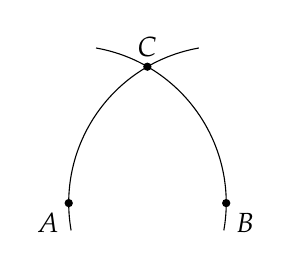
\begin{tikzpicture}[scale=0.5]
\coordinate (A) at (0,0);
\coordinate (B) at (4,0);
\path (A) node[below left] {$A$} -- (B) node[below right] {$B$};
\fill (A) circle[radius=3pt];
\fill (B) circle[radius=3pt];
\draw[name path=larc] (A) ++(-10:4cm) arc (-10:80:4cm);
\draw[name path=rarc] (B) ++(-170:4cm) arc (-170:-260:4cm);
\path [name intersections={of=larc and rarc,by={t}}];
\fill (t) node[above] {$C$} circle[radius=3pt];
\end{tikzpicture}
\caption{Constructing an equilateral triange using only a compass.}\label{fig.mm}
\end{center}
\end{figure}
\vspace*{-4ex}
\item  A straightedge alone cannot construct everything that can be constructed with a straightedge and compass, but all such constructions can be done if in addition to the straightedge there is a single circle centered at an arbitrary position in the plane with an arbitrary radius. This theorem was proved by Jacob Steiner in 1833.
\end{itemize}
The proofs of these theorems are somewhat long but not very difficult. They can be found in the book by Heinrich D\"{o}rrie \cite{dorrie1}, which is more accessible in a new edition \cite{dorrie2}.

In the other direction, Greek mathematicians investigated constructions using tools that are more complex that an (unmarked) straightedge and a compass. In the 19th century it was proved that an angle cannot be trisected (divided into three equal parts) using a straightedge and compass. However, trisecting an angle is possible using a \emph{neusis}, a straightedge with two marks on it, or a \emph{quadratix} which is built from two straightedges connected so that they can slide and rotate. I have written a document presenting these constructions: ``How to trisect an angle (if you are willing to cheat),'' which can be found on my website at \url{http://www.weizmann.ac.il/sci-tea/benari/mathematics}.


%%%%%%%%%%%%%%%%%%%%%%%%%%%%%%%%%%%%%%%%%%%%%%%%%%%%%%%%%%%%%%%

\section{Don't trust a diagram}

In Section~\ref{s.erroneous}, we saw that a diagram can lead us astray. To emphasize this point, I now present a proof that \emph{all} triangles are isosceles!

Given an arbitrary triangle $\triangle ABC$, let $P$ be the intersection of the angle bisector of $\angle A$ and the perpendicular bisector $DP$ of $BC$ (Figure~\ref{fig.isosceles}). $E,F$ are the intersections of perpendiculars from $P$ to the other two sides $AB,AC$.
\begin{figure}[H]
\begin{center}
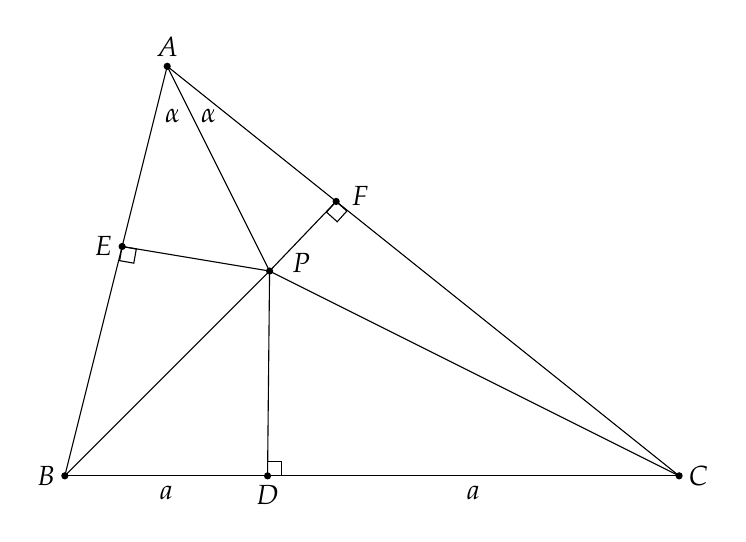
\begin{tikzpicture}[scale=1.3]
\coordinate (P) at (0,0);
\node[xshift=4mm,yshift=1mm] at (P) {$P$};
\coordinate [label=left:$B$] (B)  at (-2,-2);
\coordinate [label=right:$C$] (C)  at (4,-2);
\coordinate [label=above:$A$] (A)  at (-1,2);
\node[below,yshift=-12pt,xshift=2pt] at (A) {$\alpha$};
\node[below,yshift=-12pt,xshift=15pt] at (A) {$\alpha$};
\draw (A) -- (B);
\draw (A) -- (C);
\draw (B) -- (C);
\draw (A) -- (P);
\draw (B) -- (P);
\draw (C) -- (P);
\coordinate[label=left:$E$] (E) at ($ (A) ! .44 ! (B) $);
\draw[rotate=-100] (E) rectangle +(4pt,4pt);
\draw (P) -- (E);
\coordinate (F) at ($ (A) ! .33 ! (C) $);
\node[right,xshift=2pt,yshift=2pt] at (F) {$F$};
\draw[rotate=-132] (F) rectangle +(4pt,4pt);
\draw (P) -- (F);
\coordinate[label=below:$D$] (D) at ($ (B) ! .33 ! (C) $);
\draw (D) rectangle +(4pt,4pt);
\draw (P) -- (D);
\node[left] at ($ (A) ! .5 ! (E) $) {};
\node[left] at ($ (B) ! .5 ! (E) $) {};
\node[below] at ($ (B) ! .5 ! (D) $) {$a$};
\node[below] at ($ (C) ! .5 ! (D) $) {$a$};
\node[right,xshift=2pt] at ($ (A) ! .5 ! (F) $) {};
\node[right,xshift=2pt] at ($ (C) ! .5 ! (F) $) {};
\foreach \n in {A,B,C,D,E,F,P} {
  \fill (\n) circle[radius=1pt];
}
\end{tikzpicture}
\caption{All triangles are isosceles}\label{fig.isosceles}
\end{center}
\end{figure}
\vspace*{-4ex}
The triangles $\triangle APF, \triangle APE$ are right triangles with equal angle $\alpha$ and a common side $AP$. Therefore, they are congruent by angle-angle-side. $PD$ is perpendicular bisector so $DC=BD$; since $PD$ is a common side, the right triangles $\triangle DPC, \triangle DPB$ are congruent by side-angle-side and we conclude that $BP=PC$. We have already shown that $\triangle APF, \triangle APE$ are congruent so $EP=FP$; therefore, $\triangle EPB, \triangle EPC$ are congruent since they are both right triangles with two sides known. (The third side can be calculated by Pythagoras' Theorem, so they are congruent by side-side-side.) It follows that $EB=FC$. We conclude that $AB= AE+EB=AF+FC =AC$ and the triangle $\triangle ABC$ is isosceles.

The proof is \emph{correct} but the diagram is not. I have prepared a GeoGebra file \texttt{isosceles.ggb} which shows a triangle for which the point $P$ is \emph{outside} the triangle.


%%%%%%%%%%%%%%%%%%%%%%%%%%%%%%%%%%%%%%%%%%%%%%%%%%%%%%%%%%%%%%%

\newpage

\bibliographystyle{plain}
\bibliography{compass}

\end{document}
